\section{Räumliche Faltung}
\label{raeumliche_faltung}

Der räumliche Faltungsoperator von~\citeauthor{patchy} hat das Ziel, den Graphen in einen dreidimensionalen Tensor zu konvertieren, sodass die klassische Faltungsoperation \gls{conv2d} auf diesen angewendet werden kann.
Der Prozess zur \emph{Vektorisierung} eines Graphen besteht dabei aus drei Schritten: (1) Bestimme eine Auswahl $\gls{V}_{\mathrm{out}} \subseteq \gls{V}$, $\left|\gls{V}_{\mathrm{out}}\right| = L$, der Knoten des Graphen $\gls{G} = \left(\gls{V}, \gls{E}\right)$ mit einer zuvor definierten Länge $L \in \gls{N}$, (2) finde für jeden ausgewählten Knoten $\gls{v} \in \gls{V}_{\mathrm{out}}$ eine Nachbarschaftsgruppierung $\gls{Neighbor}_{\gls{v}} \subseteq \gls{V}$, (3) normalisiere die jeweiligen Nachbarschaften $\gls{Neighbor}_{\gls{v}}$ auf eine festgelegte Größe $K \in \gls{N}$ zu $\gls{Neighbor}_{\mathrm{out}}$, $\left|\gls{Neighbor}_{\mathrm{out}}\right| = K$, und bestimme auf diesen eine Ordnung, sodass Graphen mit ähnlichen Nachbarschaftsstrukturen eine äquivalente Ordnung erzeugen~\cite{patchy}.
Im Folgenden werden die drei Schritte näher erläutert.

\paragraph{Knotenauswahl}
\label{knotenauswahl}

\begin{algorithm}[t]
\centering
\begin{algorithmic}
  \REQUIRE{} Knotenmenge \gls{V}, Färbung $\gls{l} \colon \gls{V} \to \gls{C} \subseteq \gls{R}$, Länge $L \in \gls{N}$, Schrittweite $S \in \gls{N}$
  \ENSURE{} geordnete Knotenmenge $\gls{V}_{\mathrm{out}} \subseteq \gls{V}$ mit $\left|\gls{V}_{\mathrm{out}}\right| \leq l$
  \STATE{} $\gls{V}_\mathrm{out} \leftarrow \left[\,\,\right]$
  \STATE{} $\gls{V}_{\mathrm{sort}} \leftarrow$ Sortiere \gls{V} absteigend \bzgl{} \gls{l}.
  \STATE{} $i, j \leftarrow 1$
  \WHILE{$i < L$}
    \IF{$j \leq \left|\gls{V}_{\mathrm{sort}}\right|$}
      \STATE{} $\gls{V}_{\mathrm{out}}\left[i\right] \leftarrow \gls{V}_{\mathrm{sort}}\left[j\right]$
    \ENDIF{}
    \STATE{} $i \leftarrow i + 1$
    \STATE{} $j \leftarrow j + S$
  \ENDWHILE{}
  \RETURN{$\gls{V}_{\mathrm{out}}$}
\end{algorithmic}
\caption[Knotenauswahl]{Berechnung der Knotenauswahl $\gls{V}_{\mathrm{out}}$ anhand einer Knotenfärbung $\gls{l} \colon \gls{V} \to \gls{C} \subseteq \gls{R}$, einer maximalen Länge $L\in\gls{N}$ sowie einer Schrittweite $S \in \gls{N}$.}
\label{alg:knotenauswahl}
\end{algorithm}

Die Knotenauswahl beschreibt den Prozess zur Auswahl einer geordneten Teilmenge $\gls{V}_{\mathrm{out}} \subseteq \gls{V}$ mit nicht mehr als $L \in \gls{N}$ vielen Knoten, für die im späteren Verlauf eine Nachbarschaft des Graphen \bzw{} ein Receptive-Field des Netzes erzeugt wird~\cite{patchy}.
Algorithmus~\ref{alg:knotenauswahl} veranschaulicht die grobe Vorgehensweise dieses Verfahrens.
Dafür werden anhand einer gegebenen Knotenfärbung $\gls{l} \colon \gls{V} \to \gls{C} \subseteq \gls{R}$ die Knoten in \gls{V} absteigend sortiert, sodass Knoten, die aufgrund ihrer Zentralität als wichtiger gelten, am Anfang der geordneten Knotenmenge $\gls{V}_{\mathrm{sort}}$ stehen.
Folglich kann über die geordnete Knotenmenge $\gls{V}_{\mathrm{sort}}$ iteriert werden und in Abständen \bzw{} Schrittweiten $S \in \gls{N}$ solange Knoten aus $\gls{V}_{\mathrm{sort}}$ entnommen werden, bis $L$ viele gefunden wurden oder die Menge zu Ende iteriert wurde.
$S$ gibt damit den Abstand zweier benachbarter Knoten in $\gls{V}_{\mathrm{out}}$ an, für die ein Receptive-Field generiert wird.
Falls die Liste eine kleinere Anzahl an Knoten als $S\left( L -1 \right) + 1$ besitzt, dann besitzt $\gls{V}_{\mathrm{out}}$ folglich eine Kardinalität kleiner als $L$.
Demnach ist es möglich, dass $\gls{V}_{\mathrm{out}}$ weniger, aber niemals mehr Knoten als $L$ enthält (\vgl{}~\cite{patchy}).

\paragraph{Nachbarschaftsgruppierung}
\label{nachbarschaftsgruppierung}

\begin{algorithm}[t]
\centering
\begin{algorithmic}
  \REQUIRE{} Knoten $\gls{v} \in \gls{V}_{\mathrm{out}}$, Receptive-Field-Größe $K \in \gls{N}$
  \ENSURE{} Nachbarschaftsmenge $\gls{Neighbor}_{\gls{v}} \subseteq \gls{V}$
  \STATE{} $\gls{Neighbor}_{\gls{v}}, \mathcal{T} \leftarrow \left\{\gls{v}\right\}$
  \WHILE{$\left|\gls{Neighbor}_{\gls{v}}\right| < K$ und $\left|\mathcal{T}\right| > 0$}
    \STATE{} $\mathcal{T} \leftarrow \bigcup_{\gls{v} \in \mathcal{T}} \gls{Neighbor}\left(\gls{v}, 1\right)$
    \STATE{} $\gls{Neighbor}_{\gls{v}} \leftarrow \gls{Neighbor}_{\gls{v}} \cup \mathcal{T}$
  \ENDWHILE{}
  \RETURN{$\gls{Neighbor}_{\gls{v}}$}
\end{algorithmic}
\caption[Nachbarschaftsgruppierung]{Berechnung einer Vorauswahl der maximal in dem Receptive-Field des Knotens $\gls{v} \in \gls{V}_{\mathrm{out}}$ mit Größe $K \in \gls{N}$ enthaltenden Knoten über eine von \gls{v} ausgehende Breitensuche.}
\label{alg:nachbarschaftsgruppierung}
\end{algorithm}

Für jeden in $\gls{V}_{\mathrm{out}} \subseteq \gls{V}$ enthaltenden Knoten muss nun ein Receptive-Field konstruiert werden.
Dafür generiert Algorithmus~\ref{alg:nachbarschaftsgruppierung} zuvor eine Nachbarschaftsgruppierung $\gls{Neighbor}_{\gls{v}} \subseteq \gls{V}$ eines jeden Knoten $\gls{v} \in \gls{V}_{\mathrm{out}}$, die eine Vorauswahl der maximal in dessen Receptive-Field enthaltenden Knoten beschreibt.
Für einen Knoten $\gls{v} \in \gls{V}_{\mathrm{out}}$ und eine Receptive-Field-Größe $K \in \gls{N}$ vollzieht der Algorithmus eine von $v$ ausgehende Breitensuche durch den Graphen, bei der die Knoten in Abhängigkeit zu ihrem Abstand zu \gls{v} durchlaufen werden.
Dabei werden zuerst die lokalen Nachbarknoten $\gls{v}_i \in \gls{V}$ mit $\left(\gls{v}, \gls{v}_i\right) \in \gls{E}$ zu der Menge $\gls{Neighbor}_{\gls{v}} \in \gls{V}$ hinzugefügt.
Falls $\left|\gls{Neighbor}_{\gls{v}}\right| < K$ werden die Nachbarschaften der zuletzt zu $\gls{Neighbor}_{\gls{v}}$ hinzugefügten Knoten durchlaufen und zu $\gls{Neighbor}_{\gls{v}}$ hinzugefügt.
Der Prozess wiederholt sich solange, bis mindestens $K$ Knoten gefunden wurden oder keine Knoten mehr zur Verfügung stehen, für die ein Weg nach \gls{v} existiert und noch nicht in der Nachbarschaftsgruppierung enthalten sind.
$\gls{Neighbor}_{\mathrm{v}}$ erzeugt dabei in den allermeisten Fällen eine Menge, die sich in ihrer Anzahl stark von $K$ unterscheidet (\vgl{}~\cite{patchy}).

\paragraph{Normalisierung}
\label{normalisierung}

Die Nachbarschaftsgruppierung $\gls{Neighbor}_{\gls{v}}$ eines Knoten $\gls{v} \in \gls{V}_{\mathrm{out}}$ wird im Anschluss darauf zu einem Receptive-Field $\gls{Neighbor}_{\mathrm{out}}$ mit einer festen Größe $\left|\gls{Neighbor}_{\mathrm{out}}\right| = K$ und einer totalen Ordnung auf dessen Elementen \emph{normalisiert}, sodass Knoten in zwei verschiedenen Graphen genau dann an eine ähnliche Position im Receptive-Field gelangen, wenn sich ihre strukturellen Rollen in den Graphen ähneln~\cite{patchy}.
Die Normalisierung ist damit ein Prozess, der eine ungeordnete Knotenmenge in einen Vektorraum mit linearer Ordnung transformiert~\cite{patchy}.

\begin{algorithm}[t]
\centering
\begin{algorithmic}
  \REQUIRE{} Graph \gls{G}, Knoten $\gls{v} \in \gls{V}_{\mathrm{out}}$, Nachbarschaftsmenge $\gls{Neighbor}_{\gls{v}} \subseteq \gls{V}$, Receptive-Field-Größe $K \in \gls{N}$, Färbung $\gls{l} \colon \gls{V} \to \gls{C} \subseteq \gls{R}$
  \ENSURE{} geordnete Nachbarschaftsmenge $\gls{Neighbor}_{\mathrm{out}}$ mit $\left|\gls{Neighbor}_{\mathrm{out}}\right| = K$
  \STATE{} berechne Ordnung $>_{\gls{v}}$, sodass $\gls{v}_i >_{\gls{v}} \gls{v}_j$ \gdw{} $\gls{s}\left(\gls{v}, \gls{v}_i\right) > \gls{s}\left(\gls{v}, \gls{v}_j\right)$ und $\gls{l}\left(\gls{v}_i\right) < \gls{l}\left(\gls{v}_j\right)$ falls $\gls{s}\left(\gls{v}, \gls{v}_i\right) = \gls{s}\left(\gls{v}, \gls{v}_j\right)$.
  \STATE{} $\gls{Neighbor}_{\mathrm{sort}} \leftarrow$ Sortiere $\gls{Neighbor}_{\gls{v}}$ aufsteigend \bzgl{} $>_{\gls{v}}$.
  \IF{$\left|\gls{Neighbor}_{\gls{v}}\right| > K$}
    \STATE{} $\gls{Neighbor}_{\mathrm{sort}} \leftarrow \gls{Neighbor}_{\mathrm{sort}}\left[0:K\right]$
  \ENDIF{}
  \STATE{} $\gls{G}^{\prime} = \left(\gls{V}^{\prime}, \gls{E}^{\prime}\right) \leftarrow$ Generiere Teilgraph aus \gls{G} mit Knotenmenge $\gls{V}^{\prime} \coloneqq \gls{Neighbor}_{\mathrm{sort}} \subseteq \gls{V}$.
  \STATE{} $\gls{Neighbor}_{\mathrm{out}} \leftarrow$ Kanonisiere $\gls{G}^{\prime}$ \bzgl{} $>_{\gls{v}}$ (hebt Gleichheiten in $>_{\gls{v}}$ auf).
  \RETURN{$\gls{Neighbor}_{\mathrm{out}} \cup \left(\max \left(K - \left|\gls{Neighbor}_{\gls{v}}\right|, 0\right) \text{ Fakeknoten}\right)$}
\end{algorithmic}
\caption[Normalisierung]{Berechnung der Vektorrepräsentation einer Nachbarschaftsmenge $\gls{Neighbor}_{\gls{v}}$ eines Knotens $\gls{v} \in \gls{V}_{\mathrm{out}}$ mittels einer vordefinierten Größe $K \in \gls{N}$, einer Färbung $\gls{l} \colon \gls{V} \to \gls{C} \subseteq \gls{R}$ sowie der Abstandsfunktion $\gls{s} \colon \gls{V} \times \gls{V} \to \gls{N}$ des Graphen \gls{G}.}
\label{alg:normalisierung}
\end{algorithm}

Algorithmus~\ref{alg:normalisierung} veranschaulicht den von \citeauthor{patchy} entwickelten Normalisierungsprozess \bzgl{} eines Knotens $\gls{v} \in \gls{V}_{\mathrm{out}}$ basierend auf dessen zuvor ermittelter Nachbarschaftsmenge $\gls{Neighbor}_{\gls{v}}$.
Dafür werden die Knoten der Nachbarschaftsmenge $\gls{v}_i \in \gls{Neighbor}_{\gls{v}}$ zuerst aufsteigend \bzgl{} ihrer Abstände $\gls{s}\left(\gls{v}, \gls{v}_i\right)$ zu \gls{v} und absteigend \bzgl{} ihrer jeweiligen Knotenfarbe bei gleichen Abständen sortiert.
Falls $\gls{v}_i$ näher an \gls{v} als $\gls{v}_j$ liegt, \dhe{} $\gls{s}\left(\gls{v}, \gls{v}_i\right) < \gls{s}\left(\gls{v}, \gls{v}_j\right)$, befindet sich $\gls{v}_i$ immer vor $\gls{v}_j$ in der resultierenden normalisierten Nachbarschaftsmenge $\gls{Neighbor}_{\mathrm{out}}$.
Damit befindet sich der Wurzelknoten \gls{v} stets an erster Position in $\gls{Neighbor}_{\mathrm{out}}$ und je weiter ein Knoten von \gls{v} entfernt liegt, umso höher ist sein Index in der Vektorrepräsentation.
Anschließend kann die ermittelte Sortierung auf die Größe $K$ reduziert werden, indem die Elemente ab der Position $K+1$ verworfen werden.

Da die meisten Knotenfärbungsalgorithmen \gls{l} nicht injektiv sind und daher möglicherweise auf die gleiche Farbe innerhalb einer \enquote{Abstandsgruppe} abbilden, ist die generierte Sortierung $\gls{Neighbor}_{\mathrm{sort}}$ insbesondere nicht total.
Es ist daher notwendig, die Äquivalenzen dieser Knotenfarbe aufzulösen.
Für diesen Zweck wird ein Teilgraph $\gls{G}^{\prime} = \left(\gls{V}^{\prime}, \gls{E}^{\prime}\right)$ aus \gls{G} generiert, der \gls{G} auf die Nachbarschaftsmenge $\gls{V}^{\prime} \coloneqq \gls{Neighbor}_{\mathrm{sort}}$ beschränkt.
Eine kanonische Ordnung auf diesem Graphen mit Berücksichtigung der Knotenfärbung \gls{l} liefert damit eine totale Ordnung der Knoten in $\gls{Neighbor}_{\mathrm{sort}}$ mit gleicher Knotenfarbe.
Eine kanonische Ordnung auf Graphen mit fester Größe $K$ ist dabei in linearer Zeit möglich (\vgl{}~\cite{patchy}).
Da die Kanonisierung des Graphen nur für Knoten mit gleicher Knotenfarbe angewendet werden muss, zeigt sich der zusätzliche Aufwand dieser Operation als zu vernachlässigen.

Abschließend muss weiterhin der Fall betrachtet werden, dass $\left|\gls{Neighbor}_{\gls{v}}\right| < K$ weniger als $K$ Knoten enthält.
Dafür werden $\max\left(K - \left|\gls{Neighbor}_{\gls{v}}\right|, 0\right)$ \emph{Fakeknoten} an das Ende von $\gls{Neighbor}_{\mathrm{out}}$ gehängt, denen keine Bedeutung innewohnt und später so belegt werden, dass diese keinen Einfluss auf das Resultat der Faltung nehmen.
\begin{figure}[t]
\centering
  \subfigure[$\gls{G}^{\prime} = \left(\gls{Neighbor}_{\gls{v}}, \gls{E}^{\prime}\right)$]{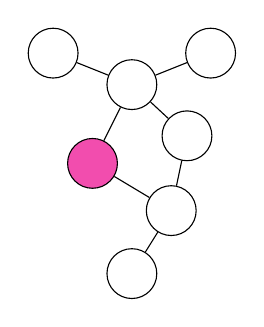
\begin{tikzpicture}
  \tikzstyle{node}=[circle,draw, minimum width=18pt, inner sep=0pt, fill=white]
  \tikzstyle{root}=[fill=magenta!70]

  \node[node, root] (1) at (0,    0)    {};
  \node[node]       (2) at (0.5,  1)    {};
  \node[node]       (3) at (1,    -0.6) {};
  \node[node]       (4) at (1.2,  0.35) {};
  \node[node]       (5) at (1.5,  1.4)  {};
  \node[node]       (6) at (-0.5, 1.4)  {};
  \node[node]       (7) at (0.5,  -1.4) {};

  \path (1) edge (2);
  \path (1) edge (3);
  \path (2) edge (4);
  \path (2) edge (5);
  \path (2) edge (6);
  \path (3) edge (4);
  \path (3) edge (7);
\end{tikzpicture}
}
\hspace{1cm}
  \subfigure[Distanz]{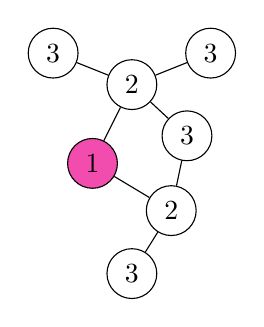
\begin{tikzpicture}
  \tikzstyle{node}=[circle,draw, minimum width=18pt, inner sep=0pt, fill=white]
  \tikzstyle{root}=[fill=magenta!70]

  \node[node, root] (1) at (0,    0)    {$1$};
  \node[node]       (2) at (0.5,  1)    {$2$};
  \node[node]       (3) at (1,    -0.6) {$2$};
  \node[node]       (4) at (1.2,  0.35) {$3$};
  \node[node]       (5) at (1.5,  1.4)  {$3$};
  \node[node]       (6) at (-0.5, 1.4)  {$3$};
  \node[node]       (7) at (0.5,  -1.4) {$3$};

  \path (1) edge (2);
  \path (1) edge (3);
  \path (2) edge (4);
  \path (2) edge (5);
  \path (2) edge (6);
  \path (3) edge (4);
  \path (3) edge (7);
\end{tikzpicture}
}
\hspace{1cm}
  \subfigure[Zentralität]{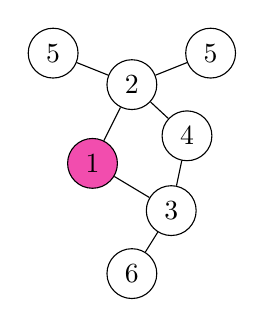
\begin{tikzpicture}
  \tikzstyle{node}=[circle,draw, minimum width=18pt, inner sep=0pt, fill=white]
  \tikzstyle{root}=[fill=magenta!70]

  \node[node, root] (1) at (0,    0)    {$1$};
  \node[node]       (2) at (0.5,  1)    {$2$};
  \node[node]       (3) at (1,    -0.6) {$3$};
  \node[node]       (4) at (1.2,  0.35) {$4$};
  \node[node]       (5) at (1.5,  1.4)  {$5$};
  \node[node]       (6) at (-0.5, 1.4)  {$5$};
  \node[node]       (7) at (0.5,  -1.4) {$6$};

  \path (1) edge (2);
  \path (1) edge (3);
  \path (2) edge (4);
  \path (2) edge (5);
  \path (2) edge (6);
  \path (3) edge (4);
  \path (3) edge (7);
\end{tikzpicture}
}
\hspace{0.6cm}
  \subfigure[Kanonisierung]{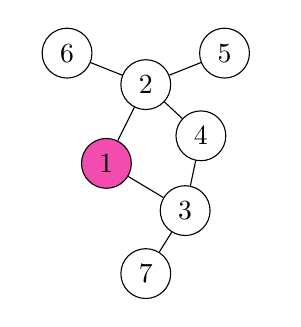
\begin{tikzpicture}
  \fill [white] (-1, 0) rectangle (2, 1) node {};  % Zentriere Graph.
  \tikzstyle{node}=[circle,draw, minimum width=18pt, inner sep=0pt, fill=white]
  \tikzstyle{root}=[fill=magenta!70]

  \node[node, root] (1) at (0,    0)    {$1$};
  \node[node]       (2) at (0.5,  1)    {$2$};
  \node[node]       (3) at (1,    -0.6) {$3$};
  \node[node]       (4) at (1.2,  0.35) {$4$};
  \node[node]       (5) at (1.5,  1.4)  {$5$};
  \node[node]       (6) at (-0.5, 1.4)  {$6$};
  \node[node]       (7) at (0.5,  -1.4) {$7$};

  \path (1) edge (2);
  \path (1) edge (3);
  \path (2) edge (4);
  \path (2) edge (5);
  \path (2) edge (6);
  \path (3) edge (4);
  \path (3) edge (7);
\end{tikzpicture}
}
\caption[Normalisierung]{Illustration der Normalisierung einer Nachbarschaft eines Knotens (rot) mit $7$ Knoten (a) zur Bestimmung einer eindeutigen Anordnung dieser.
Dazu werden die Nachbarschaftsknoten zuerst auf Basis ihrer Distanz zum Wurzelknoten gruppiert (b).
Innerhalb einer Gruppierung werden die Knoten auf Basis einer gegebenen Zentralitätsmetrik sortiert (c).
Im Anschluss werden Äquivalenzen in der Zentralität innerhalb einer Gruppe über dessen kanonische Ordnung aufgelöst (d).
Gegebenenfalls muss die gefundene Ordnung auf die gewünschte Größe des Receptive-Fields zugeschnitten oder um Fakeknoten erweitert werden.}
\label{fig:raeumliche_faltung}
\end{figure}

Abbildung~\ref{fig:raeumliche_faltung} illustriert den Normalisierungsprozess an einem einfachen Beispiel.
\\\\
Für jeden Graphen \gls{G} kann damit ein dreidimensionaler Tensor $\ma{T} \in \gls{R}^{L \times K \times M}$ über die drei beschriebenen Schritte mit Hilfe einer Merkmalsmatrix $\gls{F} \in \gls{R}^{N \times M}$ auf den Knoten des Graphen generiert werden.
Dafür werden $L$ Knoten des Graphen ausgewählt und für diese die entsprechenden $K$ großen Nachbarschaften \bzw{} Receptive-Fields ermittelt.
Jeder Eintrag in $\gls{Neighbor}_{\mathrm{out}}$ wird dann durch seine entsprechenden Merkmale aus \gls{F} ersetzt.
Das erlaubt die Verwendung der klassischen \gls{conv2d}-Operation im Kontext von Graphen, die auf dreidimensionalen Tensoren operiert.
Damit entspricht die Transformation eines Graphen in den Vektorraum und einer anschließenden Faltung auf dieser Repräsentation der ersten Faltungsschicht eines klassischen \glspl{CNN}.
Für eine Knotenauswahl, die weniger als $L$ Knoten ermittelt, sowie für Receptive-Fields, die Fakeknoten enthalten, werden die entsprechenden Einträge in \ma{T} über den Wert Null repräsentiert, welche somit keinen Einfluss auf die Faltung mittels \gls{conv2d} nehmen.
